% Options for packages loaded elsewhere
\PassOptionsToPackage{unicode}{hyperref}
\PassOptionsToPackage{hyphens}{url}
%
\documentclass[
]{book}
\usepackage{amsmath,amssymb}
\usepackage{lmodern}
\usepackage{iftex}
\ifPDFTeX
  \usepackage[T1]{fontenc}
  \usepackage[utf8]{inputenc}
  \usepackage{textcomp} % provide euro and other symbols
\else % if luatex or xetex
  \usepackage{unicode-math}
  \defaultfontfeatures{Scale=MatchLowercase}
  \defaultfontfeatures[\rmfamily]{Ligatures=TeX,Scale=1}
\fi
% Use upquote if available, for straight quotes in verbatim environments
\IfFileExists{upquote.sty}{\usepackage{upquote}}{}
\IfFileExists{microtype.sty}{% use microtype if available
  \usepackage[]{microtype}
  \UseMicrotypeSet[protrusion]{basicmath} % disable protrusion for tt fonts
}{}
\makeatletter
\@ifundefined{KOMAClassName}{% if non-KOMA class
  \IfFileExists{parskip.sty}{%
    \usepackage{parskip}
  }{% else
    \setlength{\parindent}{0pt}
    \setlength{\parskip}{6pt plus 2pt minus 1pt}}
}{% if KOMA class
  \KOMAoptions{parskip=half}}
\makeatother
\usepackage{xcolor}
\IfFileExists{xurl.sty}{\usepackage{xurl}}{} % add URL line breaks if available
\IfFileExists{bookmark.sty}{\usepackage{bookmark}}{\usepackage{hyperref}}
\hypersetup{
  pdftitle={A tutorial for geochemical modeling of fluid-rock interaction using GEM-Selektor and the MINES thermodynamic database},
  pdfauthor={Alexander Gysi, New Mexico Tech, USA},
  hidelinks,
  pdfcreator={LaTeX via pandoc}}
\urlstyle{same} % disable monospaced font for URLs
\usepackage{longtable,booktabs,array}
\usepackage{calc} % for calculating minipage widths
% Correct order of tables after \paragraph or \subparagraph
\usepackage{etoolbox}
\makeatletter
\patchcmd\longtable{\par}{\if@noskipsec\mbox{}\fi\par}{}{}
\makeatother
% Allow footnotes in longtable head/foot
\IfFileExists{footnotehyper.sty}{\usepackage{footnotehyper}}{\usepackage{footnote}}
\makesavenoteenv{longtable}
\usepackage{graphicx}
\makeatletter
\def\maxwidth{\ifdim\Gin@nat@width>\linewidth\linewidth\else\Gin@nat@width\fi}
\def\maxheight{\ifdim\Gin@nat@height>\textheight\textheight\else\Gin@nat@height\fi}
\makeatother
% Scale images if necessary, so that they will not overflow the page
% margins by default, and it is still possible to overwrite the defaults
% using explicit options in \includegraphics[width, height, ...]{}
\setkeys{Gin}{width=\maxwidth,height=\maxheight,keepaspectratio}
% Set default figure placement to htbp
\makeatletter
\def\fps@figure{htbp}
\makeatother
\setlength{\emergencystretch}{3em} % prevent overfull lines
\providecommand{\tightlist}{%
  \setlength{\itemsep}{0pt}\setlength{\parskip}{0pt}}
\setcounter{secnumdepth}{5}
\usepackage{booktabs}
\usepackage{amsthm}
\makeatletter
\def\thm@space@setup{%
  \thm@preskip=8pt plus 2pt minus 4pt
  \thm@postskip=\thm@preskip
}
\makeatother
\ifLuaTeX
  \usepackage{selnolig}  % disable illegal ligatures
\fi
\usepackage[]{natbib}
\bibliographystyle{apalike}

\title{A tutorial for geochemical modeling of fluid-rock interaction using GEM-Selektor and the MINES thermodynamic database}
\author{Alexander Gysi, New Mexico Tech, USA}
\date{2021-04-07}

\begin{document}
\maketitle

{
\setcounter{tocdepth}{1}
\tableofcontents
}
\hypertarget{prerequisites}{%
\chapter*{Prerequisites}\label{prerequisites}}
\addcontentsline{toc}{chapter}{Prerequisites}

GEM-Selektor (GEMS), is a numerical modeling program with a graphical user interface based on Gibbs energy minimization and permits calculating and solving fluid-rock interaction problems of interest in geochemistry.

\begin{itemize}
\item
  Installation instructions for GEMS and more information about this modeling program can be found on the GEMS team webpage: \url{http://gems.web.psi.ch/GEMS3/techinfo.html}.
\item
  Information about the MINES database and project files for the tutorials can be found under \url{https://geoinfo.nmt.edu/mines-tdb}
\end{itemize}

Collaborators:
Dmitrii Kulik (Paul Scherrer Institute), Dan Miron (Paul Scherrer Institute), and Nicole Hurtig (New Mexico Tech)

\hypertarget{intro}{%
\chapter{Create your first project in GEMS}\label{intro}}

Here we will learn how to create a new Project, the selection of thermodynamic databases, components and equations of state for your modeling project. We will also explain the project folder structure and how to install the \href{https://geoinfo.nmt.edu/mines-tdb}{MINES thermodynamic database} for modeling hydrothermal fluid-rock interaction and ore-forming processes . You will also learn how to interact basalt with water in your first equilibrium calculations.

\hypertarget{installing-the-mines-thermodynamic-database}{%
\section{Installing the MINES thermodynamic database}\label{installing-the-mines-thermodynamic-database}}

The MINES thermodynamic database can be downloaded at \url{https://geoinfo.nmt.edu/mines-tdb} (Fig. \ref{fig:fig-1}).

\begin{figure}
\includegraphics[width=0.9\linewidth]{figures/module1/fig-1} \caption{The MINES thermodynamic database webpage and files to download. Select the weblink for MINES19.}\label{fig:fig-1}
\end{figure}

\begin{itemize}
\item
  Download and unzip the DB19.default archive folder to Downloads. Select all the database files in this folder and copy them (Fig. \ref{fig:fig-2}).
\item
  Merge these database files with the Gems3-app/Resources/DB.default folder by pasting them into DB.default (Fig. \ref{fig:fig-3}).
\end{itemize}

-- In Linux this folder is in /Gems3-app/Resources/DB.default

-- In Mac OSX this folder is in /Applications/gems3 then right-click show package content and go to Contents/Resources/DB.default

-- In Windows Gems 3.7, this folder should be in GEMS370/Gems3-app/Resources/DB.default.

The folder structure of the GEMS program, independent of the operating system used, consists of two main folders:

\begin{itemize}
\tightlist
\item
  Gems3-app

  \begin{itemize}
  \tightlist
  \item
    The GEMS3-app folder contains the program resources and also a subfolder Resources/ DB.default, which will be used to copy the MINES thermodynamic database files into it.
  \end{itemize}
\item
  Library/Gems3/projects

  \begin{itemize}
  \tightlist
  \item
    The projects folder will contain all the projects you create and work on, and will also be the folder in which you can copy the tutorial folders.
  \end{itemize}
\end{itemize}

\begin{figure}
 \includegraphics[width=0.7\linewidth]{figures/module1/fig-2} \caption{Unzipped DB19.default folder and database files to copy.}\label{fig:fig-2}
 \end{figure}

\begin{figure}
\includegraphics[width=0.7\linewidth]{figures/module1/fig-3} \caption{Database files merged with the Gems3-app/Resources/DB.default folder in GEMS.}\label{fig:fig-3}
\end{figure}

\hypertarget{creating-a-new-project-from-scratch}{%
\section{Creating a new project from scratch}\label{creating-a-new-project-from-scratch}}

\begin{itemize}
\item
  Once you copied the database files, close GEMS. Open GEMS and click \texttt{New\ Project} in the Modeling Projects window. Give a name to your project (no spaces). The user interface is shown in Figure \ref{fig:fig-4}. Note if you run into display problem on high dpi screens (4K), I suggest to change the display resolution (e.g.~to 1920 x 1080) and restart gems.
\item
  In the next window, you can choose the thermodynamic database for your project. Select the database files 3rdparty/MINES and support, then deselect other databases as shown in Figure \ref{fig:fig-5}. Click \texttt{Next}.
\end{itemize}

\emph{Do not forget, you have an extensive list of minerals included in this database. Once you have gone through the tutorials and are familiar with GEMS, it is suggested that in thermodynamic database mode you switch to the \texttt{Phase} module (Fig. \ref{fig:fig-9}), and remove minerals that are not relevant for your own specific project. Also, for less advanced users, it is easiest to not use the ternary non-ideal feldspar solid solution model (ss) but only their end members (i.e., anorthite, albite and microcline).}

\begin{figure}
\includegraphics[width=0.7\linewidth]{figures/module1/fig-4} \caption{GEMS user interface showing the project window. Click on make a `New Project` and select a project name without spaces.}\label{fig:fig-4}
\end{figure}

\begin{figure}
\includegraphics[width=0.7\linewidth]{figures/module1/fig-5} \caption{Select 3rdparty/mines and support, and for phases select only withoutss. Note that we recommend only advanced users to choose withss; the expanded tab shows pure for endmembers and ss for different solid solution endmembers}\label{fig:fig-5}
\end{figure}

\begin{itemize}
\item
  In the next window choose your system components: H-O-C-Cl-Na-K-Ca-Mg-Al-Fe-Si-Ti (Fig. \ref{fig:fig-6}). Have you checked you got all of the elements selected? Check again please, then click \texttt{Next}\ldots By doing so, GEMS will automatically look up all phases with these components in the MINES database and copy them into your modeling project! \emph{Tip of the day: all your modeling projects you are working on are located under Library/Gems3/projects. Make sure to do regular backups\ldots{}}
\item
  In the next window you will be able to choose the activity model for your aqueous speciation calculations (e.g.~``Debye-Hückel'', Davies equation, \ldots), and the EOS for gases. For now, follow Figure \ref{fig:fig-7} using the extended ``Debye-Hückel'' equation (Helgeson), check the parameters and click \texttt{Check} for the aqueous speciation model. \emph{This model is ideal for modeling H\(_2\)O-NaCl aqueous solutions (with NaCl as background electrolyte) at hydrothermal conditions at relatively moderate salinities observed in many ore deposits.}
\item
  Then you can switch to the gas EOS model tab and choose the Peng-Robinson-Stryjek-Vera (PRSV) model and click \texttt{Check} (Fig. \ref{fig:fig-7}). That's it, now you are ready to model your first equilibrium model!
\end{itemize}

\emph{Note: this model is for non-ideal gases, and for this purpose a new phase with the acronym (f) was added to the MINES database with all the relevant parameters using the PRSV EOS. Else the choice would be the ideal gas law with a phase using the acronym (g)}

\begin{figure}
\includegraphics[width=0.8\linewidth]{figures/module1/fig-6} \caption{Select here the composition of the system. All phases containing these elements will automatically be loaded from the MINES database into your project.}\label{fig:fig-6}
\end{figure}

\begin{figure}
\includegraphics[width=0.7\linewidth]{figures/module1/fig-7} \caption{Select here the activity model for aqueous speciation (a-d) and the EOS model for gases (e-g).}\label{fig:fig-7}
\end{figure}

\hypertarget{your-first-fluid-rock-equilibrium-model}{%
\section{Your first fluid-rock equilibrium model}\label{your-first-fluid-rock-equilibrium-model}}

\begin{itemize}
\item
  In the next window, you will be able to define the name of your first fluid-rock system equilibrium (\texttt{SysEq}) calculations and set the pressure and temperature (Fig. \ref{fig:fig-8}).
\item
  Add a name without spaces and P-T conditions, i.e.~we choose basalt-fluid, 250 \(^{\circ}\)C for T and 1 kbar for P.
\item
  Next window we select our ingredients and add 1000 g of H\(_2\)O (Aqua), 200 g of NaCl, 5 g Gas CO\(_2\) and 500 g of basalt (Fig. \ref{fig:fig-8}). Click \texttt{OK}.
\item
  Finally, you can click on \texttt{Calculate\ BCC} followed by \texttt{Calculate\ equilibrium\ with\ GEM} as shown in (Fig. \ref{fig:fig-9}). You can easily create another system by selecting \texttt{Clone\ a\ new\ record\ from\ this\ one} and change the fluid/rock ratio or temperature and see what what happens with the results.
\end{itemize}

\begin{figure}
\includegraphics[width=0.7\linewidth]{figures/module1/fig-8} \caption{GEM-Selektor user interface showing the windows to create a new equilibrium system and define pressure (P) and temperature (T) for our first calculation.}\label{fig:fig-8}
\end{figure}

\begin{figure}
\includegraphics[width=0.7\linewidth]{figures/module1/fig-9} \caption{GEM-Selektor user interface showing how to `Calculate BCC` followed by `Calculate equilibrium with GEMS`. Also shown are the `Equilibrium Calculation` mode and the `Thermodynamic database` mode, where you can inspect the MINES database.}\label{fig:fig-9}
\end{figure}

\hypertarget{outcomes}{%
\section{Outcomes}\label{outcomes}}

Congratulations! In Module 1 you learned how to install the MINES thermodynamic database in your Resources/DB.default GEMS folder, the general folder structure of GEMS, how to setup your first project and how to run your first fluid-rock equilibrium calculations in GEMS.

\hypertarget{module2}{%
\chapter{Feldspar reaction path}\label{module2}}

In this tutorial, you will learn to model the reaction path of K-feldspar in contact with a NaCl-bearing aqueous solution and calculate the evolution of the fluid and the minerals formed as a function of increased fluid-rock interaction. You will also learn how to set up an automated cooling process simulation and plot results from multiple simulations. We will use the GEMS project file ``Module2'' that can be found either in the /Tutorial/Module2 workshop folder or download it directly \href{https://geoinfo.nmt.edu/mines-tdb/GEMS-files/Module2.zip}{here}.

\hypertarget{compute-the-chemical-equilibrium-of-single-chemical-systems-syseq}{%
\section{Compute the chemical equilibrium of single chemical systems (SysEq)}\label{compute-the-chemical-equilibrium-of-single-chemical-systems-syseq}}

\begin{figure}
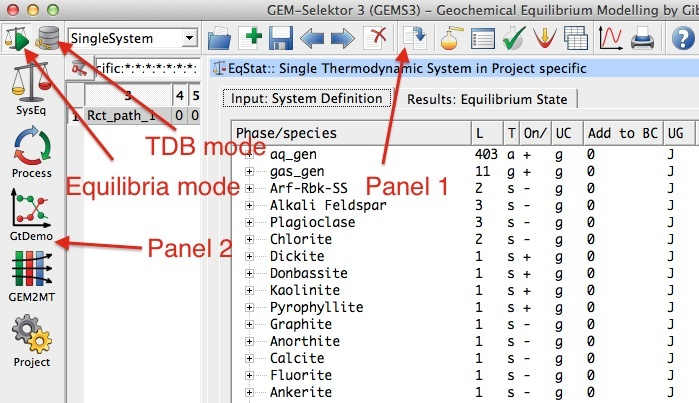
\includegraphics[width=0.7\linewidth]{figures/module2/fig-1} \caption{GEMS user interface showing the `Equilibria Calculation` and `Thermodynamic Database` modes.}\label{fig:fig-1b}
\end{figure}

\begin{itemize}
\tightlist
\item
  Copy the entire unzipped Module2 folder into your GEMS project directory located in Library/Gems3/projects. More information on the GEMS folder structure can be found in \protect\hyperlink{intro}{Module 1}.
\end{itemize}

-- For Windows users the project folder is located in C:/GEMS370/Library/Gems3/projects/ or similar.

-- For Mac OSX users, open Finder, on the top click on Go to\ldots{} and enter \textasciitilde/Library/Gems3

\begin{itemize}
\item
  Open GEMS and choose the project in the \texttt{Equilibria\ Calculation\ Mode}. The user interface is shown in Figure \ref{fig:fig-1b}. Panel 1 permits to create new records and run the program for calculations. Panel 2 gives you different calculation options.
\item
  Choose the \texttt{Create\ a\ new\ record\ from\ scratch} from the menu in Panel 1 and fill the parameters listed in Figure \ref{fig:fig-2b}
\item
  In the \texttt{Open\ recipe\ dialog}, which can also be found in Panel 1, add phases, quantity and units as shown in Figure \ref{fig:fig-3b}; Aqua (1000 g), HCl (0.1 M), NaCl (50 g), O\(_{2(g)}\) (1e-7) and K-feldspar (10 g).
\end{itemize}

\begin{figure}
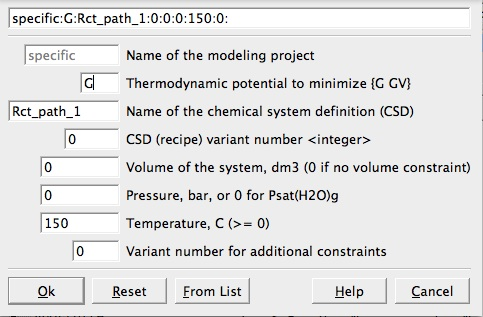
\includegraphics[width=0.7\linewidth]{figures/module2/fig-2} \caption{New record window. Select a name without spaces, a temperature and a pressure for your system. Note that a pressure of 0 corresond to saturated water vapor pressure.}\label{fig:fig-2b}
\end{figure}

\begin{figure}
\includegraphics[width=0.7\linewidth]{figures/module2/fig-3} \caption{System recipe dialog.}\label{fig:fig-3b}
\end{figure}

\begin{itemize}
\item
  Model the chemical equilibrium between 10 g of K-feldspar (microcline) and H\(_2\)O at 150 \(^\circ\)C by pressing \texttt{Calculate\ BCC} followed by \texttt{Calculate\ Equilibrium} in Panel 1. Inspect the pop up window with pH, redox (eH) and phase proportions, then accept.

  -- Determine the pH of this system as shown in the lower right of the main window (Fig. \ref{fig:fig-4b}).

  -- What is the pH of this system with 10, 20, 50 and 100 g K-feldspar? Change the amount of feldspar by clicking the \texttt{Open\ recipe\ dialog} followed by \texttt{Calculate\ BCC} and by \texttt{Calculate\ Equilibrium}. What minerals are stable with increasing pH?
\item
  Finally, clone your existing Rct\_path\_1 chemical system by selecting it and choosing \texttt{Clone\ a\ new\ record\ from\ this\ one} in Panel 1 (Fig. \ref{fig:fig-1b}). Change the name to Rct\_path\_2 and the temperature to 300 \(^\circ\)C in the pop up window, and recalculate the equilibrium of this system.

  -- Determine the pH of this system as shown in the lower right of the main window.

  -- What is the pH of this system with 10, 20, 50 and 100 g K-feldspar? What minerals are stable with increasing pH?

  -- Are there differences between the modeled system at 150 and 300 \(^\circ\)C
\end{itemize}

\begin{figure}
\includegraphics[width=0.9\linewidth]{figures/module2/fig-4} \caption{Results of the calculations, i.e. with 10 g K-feldspar added to the fluid.}\label{fig:fig-4b}
\end{figure}

\hypertarget{compute-a-titration-model-process-s-mode}{%
\section{Compute a titration model (Process, S mode)}\label{compute-a-titration-model-process-s-mode}}

The previous part of this tutorial showed you how to do individual \texttt{SysEq} calculations. What if you want to automate this process and calculate the equilibria of 10 to 100 g feldspar in steps and plot the results, i.e.~a titration model? In the following we will see how to set up \texttt{Process} simulations.

\begin{itemize}
\item
  Select the \texttt{Process} option in Panel 2 (Fig. \ref{fig:fig-1b}).
\item
  Click \texttt{Create\ a\ record\ from\ scratch} in Panel 1 and select your parent chemical system \texttt{SysEq} calculated previously at 150 \(^\circ\)C (Fig. \ref{fig:fig-5b}).
\item
  Name this process simulation ``titration\_150C'' and use the \texttt{Process\ simulation\ code} (S) as shown in Figures \ref{fig:fig-6b}) and \ref{fig:fig-7b}).
\item
  In the next window, choose a model (\texttt{titration\ cNu\ linear}), a mineral ( \texttt{Compos}, Min\_K-feldspar) and select the temperature (150 \(^\circ\)C), pressure (0 for water vapor saturation P) and amount of mineral to be added (\texttt{iNu}: 10-250 g in 10 g steps) as shown in Figure \ref{fig:fig-8b}. The parameters are: set \texttt{iTm} 1000, 1200, 1; set \texttt{iP} to 0 all fields; set \texttt{iNu} 10, 250, 10, corresponding to start, end, and step values.
\item
  Select items to be plotted (\texttt{Scalars}: pH; \texttt{Xa}: Kaolinite, Pyrophyllite, Microcline, Muscovite, Albite and Quartz) as shown in Figure \ref{fig:fig-9b}.
\item
  Accept all the following dialogues. Then click on \texttt{Save\ this\ record\ to\ database} in Panel 1, which creates your new process simulation record. Then click on the calculator icon \texttt{Re-calculate\ and\ check\ record\ data} without displaying the graph.
\end{itemize}

\begin{figure}
\includegraphics[width=0.7\linewidth]{figures/module2/fig-5} \caption{Select a parent chemical system (`SysEq`) for modeling a `Process`.}\label{fig:fig-5b}
\end{figure}
\begin{figure}
\includegraphics[width=0.7\linewidth]{figures/module2/fig-6} \caption{Name the `Process` simulator and indicate the model type (note: the process type code names are described and changeable on the next screen as well).}\label{fig:fig-6b}
\end{figure}

\begin{figure}
\includegraphics[width=0.9\linewidth]{figures/module2/fig-7} \caption{Window showing the different simulations types. Module 2 covers `mode S` for titration  or `mode P` for cooling/heating models.}\label{fig:fig-7b}
\end{figure}
\begin{figure}
\includegraphics[width=0.9\linewidth]{figures/module2/fig-8} \caption{Set the parameters for the `Process` simulation; Set `iTm` 1000, 1200, 1; Set `iP` to 0 all fields; Set `iNu` 10, 250, 10.}\label{fig:fig-8b}
\end{figure}

\begin{figure}
\includegraphics[width=0.9\linewidth]{figures/module2/fig-9} \caption{Choose the results to be plotted, including pH and mole minerals.}\label{fig:fig-9b}
\end{figure}

\begin{itemize}
\item
  There is a tab menu with 3 important selections: \texttt{Controls}, \texttt{Sampling} and \texttt{Results}. In the \texttt{Controls} tab add a description of the modeling project (Fig. \ref{fig:fig-10b}). In the \texttt{Sampling} tab change the script as shown in Figure \ref{fig:fig-11b} to choose as x-variable the amount of K-feldspar added (the process extent variable \texttt{cNu}).
\item
  Click \texttt{Save\ this\ record\ to\ database}. Toggle to the \texttt{Results} tab to inspect your modeling results. Then click on the calculator icon \texttt{Re-calculate\ and\ check\ record\ data} and check what happens with the column xp. You just assigned the \texttt{cNu} variable to the x-axis and GEMS registered it. If not, go back on the \texttt{Sampling} tab and check your script! Now lets inspect the results\ldots{}

  -- How many grams of K-feldspar need to be added to get a constant pH and what is the value?

  -- Which mineral assemblages buffer the fluid pH and can pH ranges be distinguished?
\end{itemize}

\begin{figure}
\includegraphics[width=1\linewidth]{figures/module2/fig-10} \caption{The `Controls` window showing the model conditions. The top dialog is used to add a comment and the script dialog can be customized. `iTm` is used to set the record variable; `iP` to set pressure and `iTC` temperature; `iNu` is the process variable, in this case the amount of feldspar.}\label{fig:fig-10b}
\end{figure}

\begin{figure}
\includegraphics[width=1\linewidth]{figures/module2/fig-11} \caption{The `Sampling` window showing the x- and y-axes to be sampled. Make sure to change `xp[J]` to `cNu` which is the progress variable. Then click on a blank space to make sure the script window has been registered followed by `Save this record in the database` in the top panel.}\label{fig:fig-11b}
\end{figure}

\hypertarget{modify-p-t-of-the-feldspar-reaction-path}{%
\section{Modify P-T of the feldspar reaction path}\label{modify-p-t-of-the-feldspar-reaction-path}}

Now lets clone our record to calculate the exact same titration model but changing the temperature (T) to 300 \(^\circ\)C and the pressure (P) to 500 bar.

\begin{itemize}
\item
  Clone your existing process simulation by selecting the existing record on the left and choose \texttt{Clone\ a\ new\ record}, then select your \texttt{SysEq} parent system calculated at 300 \(^\circ\)C (Fig. \ref{fig:fig-12b}). Accept all the following dialogues.
\item
  In the \texttt{Controls} tab change the description of the modeling project and change the temperature to 300 \(^\circ\)C and pressure to 500 bar to replace the starting and ending values (Fig. \ref{fig:fig-13b}). Click \texttt{Save\ this\ record\ to\ database}.
\item
  Switch the tab to \texttt{Results} and click the calculator icon \texttt{Re-calculate\ and\ check\ record\ data} to see how the pH values and moles minerals are changed by increasing the system temperature.
\item
  Toggle between both calculated process simulations at 150 and 300 \(^\circ\)C on the left pane and compare the results.
\end{itemize}

\begin{figure}
\includegraphics[width=0.7\linewidth]{figures/module2/fig-12} \caption{The `Sampling` window showing the x- and y-axes to be sampled. Make sure to change `xp[J]` to `cNu` which is the progress variable. Then click on a blank space to make sure the script window has been registered followed by `Save this record in the database` in the top panel.}\label{fig:fig-12b}
\end{figure}

\begin{figure}
\includegraphics[width=0.8\linewidth]{figures/module2/fig-13} \caption{The `Controls` window showing a model set up at a different temperture and pressure.}\label{fig:fig-13b}
\end{figure}

\hypertarget{tweak-and-plot-the-results}{%
\section{Tweak and plot the results}\label{tweak-and-plot-the-results}}

So what are the main differences for the simulations at 150 vs.~300 \(^\circ\)C? To make a better comparison lets fine tune our models and plot them!

\begin{itemize}
\item
  Select the process simulation you generated previously at 150 \(^\circ\)C and in the \texttt{Controls} tab change the amount of K-feldspar to be added using 2 to 50 g in 2 g steps and save.
\item
  Choose the \texttt{Results} tab and click the calculator icon \texttt{Re-calculate\ and\ check\ record\ data}. Click on the small \texttt{Plot\ data\ on\ Graph\ dialog} icon in Panel 1. The resulting graph should look similar to Figure \ref{fig:fig-14b}. The plots indicate that different mineral assemblages buffer the fluid pH values.
\item
  You can inspect which minerals by clicking the \texttt{Customize} button at the bottom of the plot and enter the values shown in \ref{fig:fig-15b}, then click \texttt{Apply}. Click then on \texttt{Fragment} which will enable an inset view of your plot to have a closer look at the minerals. Clicking again \texttt{Fragment} zooms out to show the pH. It is also possible to do this with the mouse, but note that this will then overwrite the x-y-axis ranges you just entered manually.
\item
  To label the lines on the plot simply drag the mineral names from the legend on the right into your plot.
\item
  You can also switch on/off minerals or pH by toggling the corresponding fields in the laegend from 0 to off (or o-letter or 0-number keys on your keyboard). Now you should be able to reproduce the look in Figure \ref{fig:fig-14b}. To save, simply click on \texttt{Save} at the bottom of your plot in the desired format (e.g.~pdf, png, etc.).
\end{itemize}

\begin{figure}
\includegraphics[width=0.8\linewidth]{figures/module2/fig-14} \caption{Simulated K-feldspar reaction path show pH and moles minerals in equilibrium with a saline aqueous fluid at 150 °C and saturated water vapor pressure.}\label{fig:fig-14b}
\end{figure}

\begin{figure}
\includegraphics[width=0.8\linewidth]{figures/module2/fig-15} \caption{`Customize` window showing options to tweak the plot. Here you can change the plot type, x- and y-axes, the font size, add labels and also the zoom-in feature by selecting x-y under Fragment. The right legend can also be turned on/off by toggling 0 to off (or using the o-letter or 0-number keys on your keyboard), and legend names dragged into the plot.}\label{fig:fig-15b}
\end{figure}

\begin{itemize}
\item
  Now select the process simulation you generated previously at 300 \(^\circ\)C and 500 bar. In the \texttt{Controls} tab change the amount of K-feldspar to be added using 5 to 125 g in 5 g steps, re-calculate and save. Try to tweak your graph to look like Figure \ref{fig:fig-16b}.
\item
  Figure \ref{fig:fig-17b} shows an alternative way to make a cumulative plot.
\item
  You can now easily compare both feldspar reaction path models generated using the \texttt{Process} simulation in S mode!
\end{itemize}

-- The resulting reaction path at 150 \(^\circ\)C is shown in Figure \ref{fig:fig-14b}.

-- The resulting reaction path at 300 \(^\circ\)C is shown in Figure \ref{fig:fig-16b}.

\begin{figure}
\includegraphics[width=0.8\linewidth]{figures/module2/fig-16} \caption{Simulated K-feldspar reaction path show pH and moles minerals in equilibrium with a saline aqueous fluid at 300 °C and 500 bar.}\label{fig:fig-16b}
\end{figure}

\begin{figure}
\includegraphics[width=0.8\linewidth]{figures/module2/fig-17} \caption{Simulated K-feldspar reaction path show pH and moles minerals in equilibrium with a saline aqueous fluid at 300 °C and 500 bar. To view this plot type choose the option `1- Cumulative` plot in the plot `Customize` window. Make sure to also switch off pH in the legend to only plot moles minerals.}\label{fig:fig-17b}
\end{figure}

\hypertarget{compute-a-cooling-model-process-p-mode}{%
\section{Compute a cooling model (Process, P mode)}\label{compute-a-cooling-model-process-p-mode}}

This part of Module 2 describes how to calculate the equilibrium between feldspar and the aqueous fluid at a constant mineral/fluid ratio but varying temperature. We will set up a cooling model from 150 to 300 \(^\circ\)C in selected steps using the \texttt{Process} simulation in \texttt{P\ mode}. We will use knowledge gained until here. This part is quick so buckle up!

\begin{itemize}
\item
  Create a parent system equilibrium record in \texttt{SysEq} simulation mode \ref{fig:fig-4b} by cloning Rct\_path\_2. Lets call this new record Rct\_cooling, select 300 °C and 500 bar, and calculate its equilibrium.
\item
  Switch to \texttt{Process}simulation mode and clone Rct\_path\_2. Select the Rct\_cooling \texttt{SysEq} record (Fig. \ref{fig:fig-18b}). Then call this new record Cooling\_150-300C and select P for the simulation mode.
\item
  In the \texttt{Controls} tab (or wizard step 2) select \texttt{No\ script}, set \texttt{iNu} to 0 and \texttt{iTC} to 300, 150, -5 as shown in Figure \ref{fig:fig-19b}.
\item
  The final step is to set the x-variable to temperature by modifying the script in the \texttt{Sampling} tab to \texttt{cTC} (Fig. \ref{fig:fig-20b}). Save your record and re-calculate.
\item
  Now you can plot and tweak your results to look similar to Figure \ref{fig:fig-21b}).
\end{itemize}

\begin{figure}
\includegraphics[width=0.7\linewidth]{figures/module2/fig-18} \caption{Select the parent record generated in `SysEq` for your new `Process` simulation.}\label{fig:fig-18b}
\end{figure}

\begin{figure}
\includegraphics[width=0.8\linewidth]{figures/module2/fig-19} \caption{`Controls` window showing the set up for a cooling model (no titration); select `No script`, set `iNu` to 0 and `iTC` to 300, 150, -5.}\label{fig:fig-19b}
\end{figure}

\begin{figure}
\includegraphics[width=0.8\linewidth]{figures/module2/fig-20} \caption{`Sampling` tab window showing how to modify the x-axis to display temperature `cTC`.}\label{fig:fig-20b}
\end{figure}

\begin{figure}
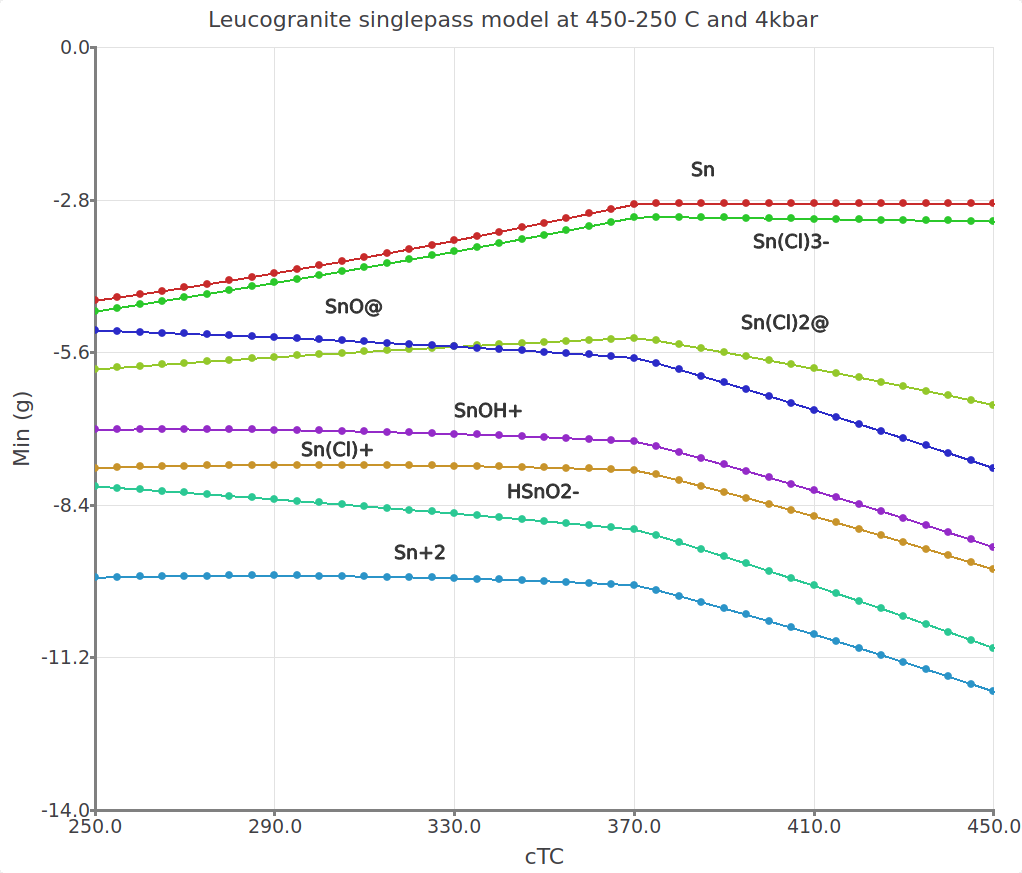
\includegraphics[width=0.8\linewidth]{figures/module2/fig-21} \caption{Cooling model showing the feldspar reaction path between 300 and 150 °C in 5 °C steps at a fluid/rock ratio of 100.}\label{fig:fig-21b}
\end{figure}

\hypertarget{outcomes-1}{%
\section{Outcomes}\label{outcomes-1}}

Good job! In Module 2 you learned how to run and automate fluid-mineral equilibria simulations using the \texttt{Process} mode. You can now generate titration models in \texttt{S\ mode} or cooling models in \texttt{P\ mode}. You also know how to do plots in GEMS, tweak and export them.

\hypertarget{module3}{%
\chapter{Greisenization Part (I)}\label{module3}}

In this module you will model the reaction path of a leucogranite during greisenization and evaluate the solubility of tin (Sn). We will learn how to: a) create \texttt{Predefined\ Composition\ Objects} (a rock or fluid composition), b) add new minerals or aqueous species to your thermodynamic database and c) simulate a more complex fluid-rock reaction path using our knowledge gained from \protect\hyperlink{module2}{Module 2}. The example follows a modeling study of the East Kemptville tin deposit from Halter et al.~(1998), Chem. Geol. 150, 1-17. We will use the GEMS project file ``Module3'' that can be found either in the /Tutorial/Module3 workshop folder or download it directly \href{https://geoinfo.nmt.edu/mines-tdb/GEMS-files/Module3.zip}{here}.

\hypertarget{create-a-custom-rock-and-fluid}{%
\section{Create a custom rock and fluid}\label{create-a-custom-rock-and-fluid}}

\begin{figure}
\includegraphics[width=1\linewidth]{figures/module3/fig-1} \caption{GEMS user interface in Thermodynamic Database Mode. For adding a fluid or a rock choose Compos in Panel 2. For adding a mineral and/or aqueous species to your database choose DComp or ReacDC in Panel 2.}\label{fig:fig-1c}
\end{figure}

\begin{itemize}
\item
  Copy the entire unzipped Module3 folder into your GEMS project directory located in Library/Gems3/projects. More information on the GEMS folder structure can be found in \protect\hyperlink{intro}{Module 1}.
\item
  Open GEMS, choose the project and switch to the \texttt{Thermodynamic\ Database\ Mode} and select in Panel 2 the option \texttt{Compos} for creating a predefined composition object (PCO). The user interface is shown in Figure \ref{fig:fig-1c}.
\item
  Select the record ``Fluid\_greisen''. In this example the fluid was already prepared for you. GEMS is versatile in the way one can add the composition of a fluid or a rock. The fluid in this example was added using independent components (\texttt{IComp}), meaning single elements. You can check this by clicking on the wrench symbol (\texttt{Remake}) and inspect the selection. It is also possible to input minerals or custom chemical formula, for example if we would like to add 1 kg of H\(_{2}\)O to this system we could define a user-defined formula; more on this later.
\item
  Data input/output windows are shown in Figure \ref{fig:fig-1c} using mole units (M). Other units such as molality (m, mol/kg H2O) or ppm can be defined. The normalization factor can be chosen so that the output windows shows the mole elements for 1 kg of substance (or adding a 0 would not yield any normalization).
\end{itemize}

\begin{figure}
\includegraphics[width=0.8\linewidth]{figures/module3/fig-2} \caption{Parameters for creating a rock as PCO.}\label{fig:fig-2c}
\end{figure}
\begin{figure}
\includegraphics[width=0.9\linewidth]{figures/module3/fig-3} \caption{Options for adding chemical components for a PCO. These include   exttt{Independent Components} (e.g. Al, K, Na),     exttt{Dependent Components} (e.g. microcline, quartz, H$_2$O) or user-defined formulae. }\label{fig:fig-3c}
\end{figure}

\begin{itemize}
\item
  To create the rock click on \texttt{Clone\ a\ new\ record} in Panel 1. Fill the parameters as shown in Figure \ref{fig:fig-2c}.
\item
  On the next dialog select ``Use formulae of Dependent Components'' (Fig. \ref{fig:fig-3c}). In the next dialog choose first independent components IComp (i.e., K, Al, Si, O, H, Na) then the dependent components \texttt{DComp}: Microcline, Muscovite, Albite and Quartz (Fig. \ref{fig:fig-4c}).
\item
  Select the \texttt{Settings} tab and fill out the amounts of \texttt{DComp} as shown in Figure \ref{fig:fig-5c}. Select the \texttt{Page\ 1} tab, add information for this PCO and normalize it to 1 kg; add zero values for \texttt{IComp}. Press \texttt{Re-calculate} in Panel 1 and save; your output results should be the same as shown in Figure \ref{fig:fig-6c}.
\end{itemize}

\begin{figure}
\includegraphics[width=0.9\linewidth]{figures/module3/fig-4} \caption{Dialog to select Dependent Components.}\label{fig:fig-4c}
\end{figure}
\begin{figure}
\includegraphics[width=0.9\linewidth]{figures/module3/fig-5} \caption{Dialog to add amounts of Dependent Components. Note the units are here in wt. percent.}\label{fig:fig-5c}
\end{figure}

\begin{figure}
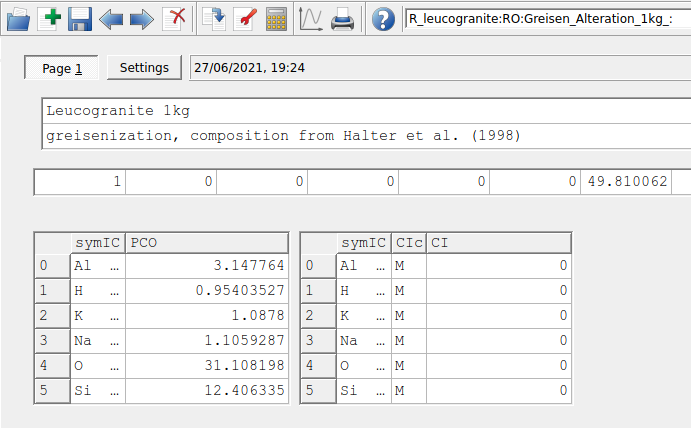
\includegraphics[width=0.9\linewidth]{figures/module3/fig-6} \caption{Dialogue to add informations on the PCO and add its normalization value (i.e., 1 kg). Make sure to put 0 values in the input window on the right side for IComp if only the input of DComp should be used for your rock composition.}\label{fig:fig-6c}
\end{figure}

\begin{itemize}
\item
  Switch to the \texttt{Equilibria\ Calculation\ Mode} (Fig. \ref{fig:fig-7c}) and stay in \texttt{SysEq} mode to calculate the equilibrium of a single system; GEMS will ask whether you want to proceed with adding the rock to your project.
\item
  Click on \texttt{Create\ a\ new\ record\ record\ from\ scratch}, give the system the following name ``Greisen\_Fl'', and a temperature of 250 \(^\circ\)C and pressure of 4000 bar.
\item
  In the \texttt{Open\ recipe\ dialog} add 200 g of rock (R\_leucogranite) and 1000 g of fluid (Fluid\_greisen). Calculate the equilibrium.
\item
  Clone this record and modify the system to 450 \(^\circ\)C and 4000 bar, calculate equilibrium.
\item
  Now lets explore the detailed results by clicking on \texttt{Open\ EqDemo\ Window\ (GEM\ task\ results)} in Panel 1 just next to the \texttt{Calculate\ Equilibrium} button. The window is shown in Figure \ref{fig:fig-8c}. Use this detailed results window to explore the following few questions:

  -- What is the pH of this system?

  -- How much Sn (molality) can you dissolve in this solution?

  -- What is the major Sn aqueous species in your model? Following the paper by Halter et al.~(1998), which Sn species might be missing in their study?

  -- Topaz is a common mineral found in Greisen. Here we only have the hydroxide (OH) endmember Topaz-OH, in the next section we will see how to add a mineral and aqueous species.
\end{itemize}

\begin{figure}
\includegraphics[width=1\linewidth]{figures/module3/fig-7} \caption{Equilibria Calculation mode with Open Recipe dialog (can be accessed by pressing on the yellow vial in Panel 1) where you can add the amounts of rock and fluid.}\label{fig:fig-7c}
\end{figure}

\begin{figure}
\includegraphics[width=1\linewidth]{figures/module3/fig-8} \caption{Open EqDemo Window (GEM task results) window: tab EqIC can be used to inspect the total dissolved molality of Sn (m\_t column); EqPh tab gives information on the mass, volume, moles and saturation index (Fa) of cassiterite (SnO2); EqDC tab shows the activities and amounts of Dependent Components, for example Sn chloride aqueous species. The EqGen gives a general overview of pH, pe, ionic strength and gas fugacities (lgFug).}\label{fig:fig-8c}
\end{figure}

\hypertarget{add-minerals-and-aqueous-species-to-database}{%
\section{Add minerals and aqueous species to database}\label{add-minerals-and-aqueous-species-to-database}}

\begin{figure}
\includegraphics[width=1\linewidth]{figures/module3/fig-9} \caption{Thermodynamic database mode showing DComp records and input fields for Topaz-F.}\label{fig:fig-9c}
\end{figure}

\begin{itemize}
\item
  Switch to the \texttt{Thermodynamic\ Database\ Mode} and select in Panel 2 (left side) the option \texttt{DComp} for adding a new mineral phase. Select the records Topaz-OH or Topaz-F and check the inputs. Figure \ref{fig:fig-9c} shows the \texttt{Page\ 1} input tab for Topaz-F. I already added this mineral for you but will briefly explain how to create such a record. Note the heat capacity function (Cp) can be set in the \texttt{Page\ 2} tab of this window.
\item
  The easiest way would be to clone an existing record, for example Topaz-OH, choose the adequate thermodynamic model for P-T corrections, and then update the thermodynamic properties (G, H, S, Cp function and V). Here few more infos:
\end{itemize}

-- Once every field is complete, click on \texttt{Re-calculate\ and\ check\ record\ data} on the top Panel 1; GEMS checks for internal consistency of your data, for example you can enter only G and S, and the program will re-calculate the H value.

-- To inspect the Topaz-F record you can select it and click on the red wrench next to the calculator on the top Panel 1. There you can explore different model options and come back to the main \texttt{DComp} window (Fig. \ref{fig:fig-9c}).

-- The top part of the window needs a mineral name and the chemical formula; the \{\} brackets are used to indicate a mixing site, i.e.~Topaz can mix OH and F on this crystallographic site.

-- Scroll through the list of mineral records, one can see that ``s'' is used for solids, ``f'' for a fluid (i.e.~non-ideal gas), and ``a'' for aqueous species. There you can explore for example the Al(OH)2+ species and see a typical set up for entering the temperature and pressure corrections for aqueous species.

\begin{figure}
\includegraphics[width=1\linewidth]{figures/module3/fig-10} \caption{Thermodynamic database mode showing the Phase records option for creating mineral. The selected record shows the input parameters for the newly created ideal solid solution between Topaz-OH and Topaz-F with (1) name of phase, (2) selected mineral endmembers of the solid solution and (3) code for defining junior and major mineral (reserved for non-ideal solid solution).}\label{fig:fig-10c}
\end{figure}

\begin{figure}
\includegraphics[width=0.7\linewidth]{figures/module3/fig-11} \caption{Datafields for creating a Phase record.}\label{fig:fig-11c}
\end{figure}

\begin{figure}
\includegraphics[width=0.7\linewidth]{figures/module3/fig-12} \caption{Selection of phase or phase endmembers for solid solutions. For a Topaz solid solution we select the OH and F endmembers}\label{fig:fig-12c}
\end{figure}

\begin{itemize}
\item
  The final step to have the new mineral phase appear in our project consists in adding a phase record in the \texttt{Phase} option (Fig. \ref{fig:fig-10c}).
\item
  Select the Topaz-OH record and click \texttt{Clone\ a\ new\ record} in Panel 1. Fill the parameters listed in Figure \ref{fig:fig-11c}.
\item
  Click next and select the mineral(s) for which you want to create a new phase. Here we select both Topaz-OH and Topaz-F for a binary solid solution (Fig. \ref{fig:fig-12c}). Note that if we would like to only add a pure phase we select only one mineral in this menu. The resulting phase record should be similar to Figure \ref{fig:fig-10c}.
\item
  The last step is to switch to the \texttt{Equilibria\ Calculation\ Mode}, accept addition of the newly created phase and re-calculate the equilibrium of your two records created previously at 250 and 450 \(^\circ\)C and 4000 bar. Now expand the Topaz solid solution, congratulation you just formed topaz! See also Figure \ref{fig:fig-13c}.
\end{itemize}

\begin{figure}
\includegraphics[width=1\linewidth]{figures/module3/fig-13} \caption{Equilibria Calculation mode showing the calculated composition of a topaz solid solution (Topaz-OH and Topaz-F).}\label{fig:fig-13c}
\end{figure}

\hypertarget{titration-of-leucogranite-to-greisen-fluid}{%
\section{Titration of leucogranite to greisen fluid}\label{titration-of-leucogranite-to-greisen-fluid}}

\begin{figure}
\includegraphics[width=0.7\linewidth]{figures/module3/fig-14} \caption{Select a parent chemical system (`SysEq`) for modeling a `Process`.}\label{fig:fig-14c}
\end{figure}

\begin{itemize}
\item
  Switch to the \texttt{Equilibria\ Calculation\ Mode}, since we have already computed a single system chemical equilibrium we can go ahead and select the option \texttt{Process} in Panel 2.
\item
  \texttt{Create\ a\ new\ record\ from\ scratch} and select ``Greisen\_Fl, 4000, 250'' as your parent chemical system record (Fig. \ref{fig:fig-14c}). Note that the parent chemical record needs to contain the fluid and the rock to be titrated with the correct units (double check in \texttt{SysEq}).
\item
  Create a titration model similar to Module 2 for the feldspar reaction path, except this time we will choose ``R\_leucogranite'' as the titrant. The simulation conditions will be 250 \(^\circ\)C and 4000 bar, and we will add 0.1 g to 2000 g of R\_leucogranite to Fluid\_greisen. Figures \ref{fig:fig-15c}, \ref{fig:fig-16c}, and \ref{fig:fig-17c} show the parameters to be entered in the subsequent \texttt{Process} wizard windows. Don't forget to un-tick the box ``Save generated SysEq records'' in Step 5 to avoid saving too many \texttt{SysEq} records.
\item
  Click \texttt{Next}, \texttt{Finish}, and save this record.
\end{itemize}

\begin{figure}
\includegraphics[width=0.7\linewidth]{figures/module3/fig-15} \caption{Name the `Process` simulator and indicate the model type.}\label{fig:fig-15c}
\end{figure}

\begin{figure}
\includegraphics[width=1\linewidth]{figures/module3/fig-16} \caption{Input parameters for a titration model of a rock (R\_leucogranite) reacting with a greisenizing fluid (Fluid\_greisen). (1) Select titration mode (Titration cNu linear), (2) titrant, (3) amount of rock to add, and (4) P-T conditions.}\label{fig:fig-16c}
\end{figure}

\begin{figure}
\includegraphics[width=1\linewidth]{figures/module3/fig-17} \caption{Choose the results to be plotted. Here we choose the mass minerals (in gram) using phM.}\label{fig:fig-17c}
\end{figure}

\begin{itemize}
\item
  Back to the main \texttt{Process} simulation window, check the \texttt{Controls} tab as shown in Figure \ref{fig:fig-18c}.
\item
  Switch to the \texttt{Sampling} window and choose cNu (i.e.~amount of rock added) instead of J as shown in Figure \ref{fig:fig-19c}. Make sure to click on an empty area outside the script box followed by save for GEMS to register the change.
\item
  Switch now to the \texttt{Results} tab, click \texttt{Re-calculate} on Panel 1 and inspect the calculated results. Make sure to save the changes.
\end{itemize}

\begin{figure}
\includegraphics[width=1\linewidth]{figures/module3/fig-18} \caption{`Controls` tab showing the parameters to set up a `Process` simulation for a titration model at 250 °C and 4kbar. Before plotting your results, (1) check you calculation control (P-T-x) script, then (2) switch the tab to `Sampling` and choose cNu for extent of reaction (amount of rock added) for the x-axis, (3) Re-calculate (numerical results can be viewed in the `Results` tab). To visualize the plot click on the plot symbol on Panel 1. To change model parameters click on Remake.}\label{fig:fig-18c}
\end{figure}

\begin{figure}
\includegraphics[width=0.8\linewidth]{figures/module3/fig-19} \caption{`Sampling` tab showing the script to extract values for the x-y axis. Change here the `xp[J]` variable to cNu, i.e. we assigned this variable to the amount of rock (R\_leucogranite) added to the system at each step. See also the script in the `Controls` window.}\label{fig:fig-19c}
\end{figure}

\begin{itemize}
\item
  Lets plot the results using the Plot dialog in Panel 1 (Fig. \ref{fig:fig-18c})
\item
  Select \texttt{Customize} at the bottom of the plot and use the parameters shown in Figure \ref{fig:fig-20c}. We can enter 0-2000 g for the x-axis and 0-815 g for the y-axis. Under \texttt{Fragment} enter 0-0.5 g for the y-axis.
\item
  The final titration models should look similar to Figures \ref{fig:fig-21c} and \ref{fig:fig-22c}. By customizing the inset view of the graph (Fragment option) it is possible to inspect the stability of cassiterite and topaz in more detail.
\item
  You can also create additional plots to investigate for example the Sn speciation, pH, etc. by cloning the existing records and change the plotting parameters. Simply click \texttt{Remake} (red wrench) in Panel 1 (Fig. \ref{fig:fig-18c}) and select the sampling parameters in Step 3 of the \texttt{Process} wizard. Additional modeling results are shown in Figure \ref{fig:fig-23c} to give you some inspiration!
\item
  Finally note: always inspect your script in the \texttt{Controls} and \texttt{Sampling} tabs to make sure your set up is ok.
\end{itemize}

-- Note what happens to cassiterite, pyrrhotite and topaz from 450 to 250 \(^\circ\)C?

-- Do you recognize different alteration styles commonly observed in ore deposits?

-- Compare your simulations to Figs. 2 and 4 in the paper from Halter et al.~(1998). What is the difference in mineralogy vs.~reaction progress (rock added)?

-- Give three factors that can affect cassiterite (SnO\(_2\)) precipitation and Sn mobility in a hydrothermal fluid.

\begin{figure}
\includegraphics[width=1\linewidth]{figures/module3/fig-20} \caption{Plot dialog showing the parameters for x-y axes for the main Graph and the inset view using Fragment. This dialog can be accessed from the `Customize` button.}\label{fig:fig-20c}
\end{figure}

\begin{figure}
\includegraphics[width=0.8\linewidth]{figures/module3/fig-21} \caption{Simulated leucogranite titration model showing the stable minerals (g) in equilibrium with a greisenizing fluid at 250 °C and 4000 bar as a function of Rock (g leucogranite) added. Comparison with Figure 2 in the Halter et al. (1998) paper indicates that our overall simulated mineralogy is similar to the progression one can expect to find in natural greisen. This progression goes from a quartz vein towards a qtz-greisen, qtz-topaz-greisen, qtz-sericite greisen, to a leucogranite.}\label{fig:fig-21c}
\end{figure}
\begin{figure}
\includegraphics[width=0.8\linewidth]{figures/module3/fig-22} \caption{Graph inset view of the leucogranite titration model at 250 °C and 4000 bar. Note certain minerals included in the calculations (e.g., magnetite and annite) were not displayed in this and previous graphs. Comparison with Halter et al. (1998) indicates that our simulated mineralogy is similar to what we find in natural greisen. The control on mineralogy can by explained by the acidity of the fluid that will also control Sn mobility. Looking at a vein alteration halo, the system changes from a fluid buffered pH (center of the quartz vein) towards a more rock buffered pH (towards the leucogranite), which is expressed in the tiration model by the increased amount of leucogranite added to the fluid (progress extent). Additional plots are necessary to show the full complexity of this system as shown below.}\label{fig:fig-22c}
\end{figure}
\begin{figure}
\includegraphics[width=0.8\linewidth]{figures/module3/fig-23} \caption{Simulated leucogranite titration model showing the log activity of aqueous Sn species vs. pH at equilibrium with a greisenizing fluid at 250 °C and 4000 bar. Similar to the feldspar reaction path (Module 2), adding rock to the fluid will lead to an increase in pH and a corresponding decrease in Sn mobility. These simulations highlight the importance of pH and salinity for the speciation of Sn and the solubility of cassiterite. }\label{fig:fig-23c}
\end{figure}

\hypertarget{outcomes-2}{%
\section{Outcomes}\label{outcomes-2}}

In this module you looked into the \texttt{Thermodynamic\ Database} mode and learned how to create a fluid and a rock (\texttt{PCO}). You also learned how to set up a \texttt{Phase} record such as a topaz solid solution and how to inspect thermodynamic data for minerals and aqueous species in \texttt{DComp}. You can now also set up different titration models with complex fluid and rock compositions, and design selected plot types for data interpretation. This module also highlights the importance of comparing the model with natural ore-forming systems.

\hypertarget{module4}{%
\chapter{Greisenization Part (II)}\label{module4}}

In this module we will continue simulating the alteration of leucogranite during greisenization and Sn mobility. You will learn how to set up an open system \texttt{Process} simulation using the single flow-through reactor (R) mode. This mode is the simplest implementation of reactive transport in one box or cell. This is generally a good start before starting more complex 1-D reactive transport simulations using sequential reactors (multiple boxes or cells) such at those implemented in the GEMS2MT module.

\begin{figure}
\includegraphics[width=1\linewidth]{figures/module4/fig-1} \caption{Conceptual models showing the two Process simulation types Leaching and Flushing in the single flow-through reactor (R) mode. }\label{fig:fig-1d}
\end{figure}

You will learn about two simulations types that can be set up in the single flow-through reactor (R) mode (from the GEMS help files):

\begin{itemize}
\item
  In the ``Leaching'' mode, at each pass (i.e.~Process step), one can follow how the solid part evolves while reacting with a ``fresh'' fluid of constant composition.
\item
  In the ``Flushing'' mode, at each pass (i.e.~Process step), one can follow how the fluid part evolves while reacting with the ``fresh'' solid part of constant composition .
\end{itemize}

We will use the GEMS project file ``Module4'' that can be found either in the /Tutorial/Module4 workshop folder or download it directly \href{https://geoinfo.nmt.edu/mines-tdb/GEMS-files/Module4.zip}{here}. Note that if you completed successfully Module 3, you can continue using this project for Module 4.

\hypertarget{multi-pass-leaching-model}{%
\section{Multi-pass (leaching) model}\label{multi-pass-leaching-model}}

A multi-pass model consists of consecutive batches of fresh (unreacted) greisen fluids (Fluid 1) reacting with a leucogranite (Rock 1) to simulate the alteration mineralogy during the formation of a hydrothermal quartz vein and alteration halo in the granite. This model can be set up using the R mode in \texttt{Process} simulation and choosing the leaching modeling scenario (Fig. \ref{fig:fig-1d}).

To set up such a model, we need a PCO for the rock (R\_leucogranite) and fluid (Fluid\_greisen), which were already prepared in Module 3, and we need to create a parent system equilibrium record.

\begin{itemize}
\tightlist
\item
  Create the parent system records in \texttt{SysEq} by cloning the two records you already created in Module 3; Greisen\_Fl records at 250 and 450 \(^\circ\)C and 4 kbar. Rename these system records to ``Rock\_leach'', and leave all the other parameters. For the input take for now 100 g of fluid and 1000 g of rock using the \texttt{Open\ recipe\ dialog} (Fig. \ref{fig:fig-2d}). Calculate the equilibrium. Save.
\end{itemize}

\begin{figure}
\includegraphics[width=1\linewidth]{figures/module4/fig-2} \caption{Create two new parent equilibrium systems containing the fluid (F-greisen 100 g) and rock (R\_leucogranite 1000 g) by cloning the Greisen\_Fl records.}\label{fig:fig-2d}
\end{figure}

\begin{itemize}
\item
  Switch to \texttt{Process} simulation and clone your record built for the titration model in Module 3. Select your parent chemical system equilibria record "Rock\textbackslash\_leach" at 450 \(^\circ\)C (Figs. \ref{fig:fig-3d}).
\item
  Name the simulation task "Rock-leaching\textbackslash\_450C" and use as simulation code R this time instead of S (Figs. \ref{fig:fig-4d} and \ref{fig:fig-5d}).
\item
  In the next window tick the option ``Leaching: Compos source'', select the fluid (Fluid\textbackslash\_greisen), then select the rock (R\textbackslash\_leucogranite) as illustrated in Figure \ref{fig:fig-6d}. Make sure to the follow the exact sequence so the script generated by the wizard will work automatically.
\item
  Click Next\ldots{} Finish.
\end{itemize}

\begin{figure}
\includegraphics[width=1\linewidth]{figures/module4/fig-3} \caption{Selection of parent system equilibrium records for setting up a new Process simulation. Note to create a new Process record clone an existing Greisen\_titration model already created in Module 3.}\label{fig:fig-3d}
\end{figure}

\begin{figure}
\includegraphics[width=0.7\linewidth]{figures/module4/fig-4} \caption{Create a new record for a Process simulation in R mode.}\label{fig:fig-4d}
\end{figure}
\begin{figure}
\includegraphics[width=0.9\linewidth]{figures/module4/fig-5} \caption{Select the simulation in R mode for setting up either a leaching or flushing models.}\label{fig:fig-5d}
\end{figure}
\begin{figure}
\includegraphics[width=1\linewidth]{figures/module4/fig-6} \caption{The Process dialogue for a multipass leaching model (mode R). To set up this system select Leaching (1), then the fluid (F\_greisen) (2) and the rock (R\_leucogranite) (3). Check that the definitions of your rock and fluid look similar to the script window (4). Select the number of fluid aliquots (5), i.e. 200 fluid aliquots (iTm: from 1000 to 1200 in steps of 1), and set P-T conditions (6). Note if we want to increase the number of fluid aliquots passing through the rock, we need to increase iTm for example from 1000 to 1400 in steps of 1 to create 400 aliquots. Also note that the fluid to rock ratio was set and can be changed in the parent SysEq record.}\label{fig:fig-6d}
\end{figure}

\begin{itemize}
\item
  Check the \texttt{Controls} window; the set up should look like Figure \ref{fig:fig-7d}.
\item
  Switch the \texttt{Sampling} tab and select the variable ``J'' for the x-axis, which represents the number of fluid aliquots passed through the rock. Click on an empty area to register the change, then save the record and click \texttt{Re-calculate}.
\item
  Plot the results and scale the x- and y-axis to inspect the results, which should look similar to Figure \ref{fig:fig-8d}. Note you can also modify the number of fluid aliquots by varying the number variable as indicated in Figure \ref{fig:fig-6d}, e.g.~instead of 200 use 400 aliquots. Do not forget you need to use \texttt{Remake} to be able to do this, as in your \texttt{Results} tab the program will need to add 200 rows in the table, which cannot be done by only changing the numbers in the ``Controls'' tab window.
\item
  Try now to change the fluid/rock ratio, for example using 1000 g fluid and 1000 g rock (f/r of 1). To do this switch to \texttt{SyEq}, select the parent record and choose 1000 g fluid and 1000 g rock, calculate the equilibrium and save. Go back to the \texttt{Process} window and re-calculate the multipass leaching model. In the pop-up window select ``Yes'' to plot the graph during the simulations!
\end{itemize}

\begin{figure}
\includegraphics[width=1\linewidth]{figures/module4/fig-7} \caption{Controls window showing the set up for a Process simulation in R mode for the leaching model at 450 °C and 4 kbar.}\label{fig:fig-7d}
\end{figure}

\begin{figure}
\includegraphics[width=1\linewidth]{figures/module4/fig-8} \caption{Simulated leucogranite multipass leaching model showing the stable minerals (g) at 450 °C and 4 kbar as a function of fluid aliquots passed through the rock. The initial fluid/rock ratio (100/1000) of 0.1.}\label{fig:fig-8d}
\end{figure}
\begin{figure}
\includegraphics[width=1\linewidth]{figures/module4/fig-9} \caption{Leucogranite multipass leaching model with a fluid/rock ratio (1000/1000) of 1.}\label{fig:fig-9d}
\end{figure}

\hypertarget{modify-p-t-of-the-leaching-model}{%
\section{Modify P-T of the leaching model}\label{modify-p-t-of-the-leaching-model}}

\begin{itemize}
\item
  To change the model temperature, we are now going to create a new "Rock\textbackslash\_leach" simulation by cloning the Process record and selecting the correspond parent chemical system at 250 °C (Fig. \ref{fig:fig-10d}).
\item
  Click next and Finish.
\item
  In the \texttt{Controls} window change the temperature to 250 °C. Make sure to save the record (Fig. \ref{fig:fig-11d}).
\item
  Click \texttt{Re-calculate} and plot the results. The simulated mineralogy should be similar to Figures \ref{fig:fig-12d} and \ref{fig:fig-13d}.
\end{itemize}

\begin{figure}
\includegraphics[width=0.7\linewidth]{figures/module4/fig-10} \caption{Selection of parent system equilibrium records for setting up a new multipass leaching model at 250 °C and 4 kbar.}\label{fig:fig-10d}
\end{figure}

\begin{figure}
\includegraphics[width=1\linewidth]{figures/module4/fig-11} \caption{Controls window showing the set up for a Process simulation in R mode for the leaching model at 250 °C and 4 kbar.}\label{fig:fig-11d}
\end{figure}

\begin{figure}
\includegraphics[width=1\linewidth]{figures/module4/fig-12} \caption{Simulated leucogranite multipass leaching model showing the stable minerals (g) at 250 °C and 4 kbar as a function of fluid aliquots passed through the rock. The initial fluid/rock ratio (100/1000) of 0.1.}\label{fig:fig-12d}
\end{figure}

\begin{figure}
\includegraphics[width=1\linewidth]{figures/module4/fig-13} \caption{Inset view showing the simulated leucogranite multipass leaching model at 250 °C and 4 kbar and initial fluid/rock ratio (100/1000) of 0.1.}\label{fig:fig-13d}
\end{figure}

\hypertarget{single-pass-flushing-and-cooling-model}{%
\section{Single-pass flushing and cooling model}\label{single-pass-flushing-and-cooling-model}}

This time we simulate the evolution of a single batch of fluid reacting progressively with more granite upon cooling and look at the evolution of the fluid composition. The conceptual model is represented by a single-pass of a fluid interacting at each step with fresh granite.

This model can also be set up using the R mode in \texttt{Process} simulation and choosing the flushing modeling scenario (Fig. \ref{fig:fig-1d}).

\begin{itemize}
\item
  Create the parent system records in \texttt{SysEq} by cloning the Rock\textbackslash\_leach model created earlier at 450 °C and 4 kbar. Rename this system records to "Rock\textbackslash\_flush", and leave all the other parameters (Fig. \ref{fig:fig-14d}).
\item
  Calculate the equilibrium. Save.
\end{itemize}

\begin{figure}
\includegraphics[width=1\linewidth]{figures/module4/fig-14} \caption{To set up a single-pass flushing model we need to create a parent chemical equilibrium system in SysEq by cloning an existing record.}\label{fig:fig-14d}
\end{figure}

\begin{itemize}
\item
  Switch to \texttt{Process} simulation and clone one of the ``Rock-leaching'' models by electing your parent record "Rock\textbackslash\_flush" created previously at 450 °C and 4 kbar (Fig. \ref{fig:fig-15d}).
\item
  Call the new record ``Rock-flushing-cool'' and use the code R for the process simulation mode (Fig. \ref{fig:fig-16d}).
\item
  Change the system parameters in the next Process wizard window to cool your system from 450 down to 250 °C at 4 kbar. Select the ``Flushing: Compos source'' model and the other options shown in Figure \ref{fig:fig-17d}. Make sure to the follow the exact sequence so the script generated by the wizard will work automatically.
\item
  In the following window select the sampling parameters. Here we will choose log of total dissolved Sn (lgm\textbackslash\_t, molality) and log activity (lga) of the aqueous Sn species as shown in Figure \ref{fig:fig-18d}.
\end{itemize}

\begin{figure}
\includegraphics[width=1\linewidth]{figures/module4/fig-15} \caption{Select the parent record Rock\_flush to create a new Process simulation by cloning on of the previously created Rock\_leaching records.}\label{fig:fig-15d}
\end{figure}

\begin{figure}
\includegraphics[width=0.7\linewidth]{figures/module4/fig-16} \caption{Input window the create a record for the flushing model.}\label{fig:fig-16d}
\end{figure}

\begin{figure}
\includegraphics[width=1\linewidth]{figures/module4/fig-17} \caption{The Process dialogue for a single-pass cooling model (R). To set up this system select Flushing (1), then the rock (2) and (3). Check that the definitions of Fluidgreisen and R\_leucogranite look similar to the script window (4). In (5) we select the temperature change between each rock column or step (i.e. from 450 to 250 °C  in -5 °C  steps). In (6) we select the number of rock columns (i.e. 40).}\label{fig:fig-17d}
\end{figure}

\begin{figure}
\includegraphics[width=1\linewidth]{figures/module4/fig-18} \caption{Sampling dialog in the Process wizard for selecting the Sn species to be plotted.}\label{fig:fig-18d}
\end{figure}

\begin{itemize}
\item
  Check the ``Sampling'' tab, if not the same use \texttt{Remake} to select the dissolved aqueous species to plot. Note for the x-axis we chose the temperature in \(^\circ\)C (cTC).
\item
  Finally, click \texttt{Re-calculate}. The results should look similar to \autoref{fig:fig11.jpeg}
\end{itemize}

\begin{figure}
\includegraphics[width=0.9\linewidth]{figures/module4/fig-19} \caption{Controls tab showing the simulation parameters for the single pass flushing and cooling model.}\label{fig:fig-19d}
\end{figure}
\begin{figure}
\includegraphics[width=0.9\linewidth]{figures/module4/fig-20} \caption{Sampling tab show the script window. Make sure to enter cTC for temperature.}\label{fig:fig-20d}
\end{figure}
\begin{figure}
\includegraphics[width=0.9\linewidth]{figures/module4/fig-21} \caption{Single-pass flushing model showing the aqueous Sn species and total dissolved Sn concentrations in a greisen fluid reacted stepwise with leucogranite and cooled from  450 to 250 °C at 4kbar.}\label{fig:fig-21d}
\end{figure}

\hypertarget{module5}{%
\chapter{GEM2MT reactive mass transport simulations of hydrothermal seawater-basalt interaction}\label{module5}}

The GEM2MT module is a tool for automation of one-dimensional (1-D) reactive mass transport simulations coupled with GEM calculation of equilibrium states in spatially distributed nodes (boxes, volumes) over time steps. GEM2MT can be used to simulate the open system evolution and fluid-rock reactions occurring along a fluid flow path (e.g.~vein, fracture, porous media, etc.). This type of simulation solves simple reactive mass transport problems, which requires the definition of fluxes between boxes of certain fluid/rock mass or volume ratios (or alternatively porosity and permeability) where fluid is moved sequentially or simultaneously from one box to the other. The GEM2MT module can simulate reactive transport in three main modes (see help file for more info):

\begin{itemize}
\tightlist
\item
  Sequential reactor chain and waves (S)
\item
  Flow-through and box-flux sequence (F, B)
\item
  One-dimensional reactive transport with advection/dispersion/diffusion (A,D,W)
\end{itemize}

To prepare for such simulations, two Compos (PCO) records are usually created in thermodynamic database mode. These two system compositions can then be copy/pasted and added later to GEM2MT, either using individual elements (Independent Components) and/or user-defined formulae units. In this example we use for Rock ``R\_Basalt'' and for Fluid ``F\_Seawater'' (already prepared in Module 5) and an example ``SWB-reactor'' was created in SysEq at 250 \(^{\circ}\)C and 500 bar.

\hypertarget{sequential-reactors-chain-s-mode}{%
\section{``Sequential reactors chain'' S mode}\label{sequential-reactors-chain-s-mode}}

In this mode, we can simulate a ``wave'' of a fluid that will pass through a series of 100 rock nodes once per step (i.e., a wave consists of ca. 100 substeps) with an initial fluid/rock ratio of 10. A schematic of the sequential reactors chain is shown in Figure \ref{fig:fig-1e}.

\begin{figure}
\includegraphics[width=0.7\linewidth]{figures/module5/fig-1} \caption{Schematic showing the sequential reactors chain (S mode). A sequence of steps forms a wave where the fluid passes and equilibrates sequentially through all of the reactors in the chain until the fluid reaches the last reactor, at which point another wave starts in the first reactor.}\label{fig:fig-1e}
\end{figure}

\begin{itemize}
\item
  Create a parent system record containing the 1000 g of the fluid and 100 g of the rock in SysEq at the temperature and pressure of interest (i.e.~250 \(^{\circ}\)C and 500 bar). This record will have to be selected when creating a new GEM2MT record (object) containing all the phases and elements relevant to the fluid-rock system of interest. Lets call this system ``SWB\_gem2mt''.
\item
  Switch to the GEM2MT module and create a new record. Select the parent system containing the rock and the fluid created above. Call this record ``sequential-reactor''
\item
  In Step 1 of the wizard, select the S mode.
\item
  In Step 2 of the wizard, set the number of nodes (nC= 101) and the maximum number of steps (in this case, ``waves'', i.e.~1000). Select 2 for the number of initial chemical system recipes, which will allow us to define the initial compositions and masses of the fluid and rock initial systems. \emph{Optionally, we can set the number of user-defined formula units that will be used for augmenting initial bulk elemental compositions of the fluid and the rock.}
\item
  In Step 3, we select ``Move aqueous fluid''.
\item
  In Step 4, we select P, T, V, Initial system, Node type, MPG flux, and Initial mass.
\item
  In Step 5, we select the variables you want to plot in each node after each ``wave''. Under n1vPH (volumes of minerals) select Cpx, Chlorite, Epidote, Calcite, Albite, Quartz, Prehnite, Wairakite, Anhydrite, Pyrite.
\end{itemize}

\begin{figure}
\includegraphics[width=9\linewidth]{figures/module5/fig-2} \caption{GEM2MT module Initial window page showing the steps to set up 1) the initial name of rock and fluid, 2) pressure and temperature, 3) input quantity of rock and fluid in kg, 4) compositions of rock and fluid (i.e., row index 0 corresponds to the fluid and row index 1 to rock), and 5) input of additional user-defined formulae and units (these fields can be added/selected in the wizard window).}\label{fig:fig-2e}
\end{figure}

After completing the wizard, we get to the GEM2MT module window ``Initial'' page (Fig. \ref{fig:fig-2e}). There we need to enter a comment about the simulation, the names of rock and fluid, temperature, pressure, mass of fluid and rock, and the initial composition of the fluid and the rock.

\begin{itemize}
\item
  In the first row (index 0), enter the name of system ``Fluid'' or similar, and add a mass of 1 kg. In the second row (index 1), enter the name of system ``Rock'' or similar, and add a mass of 0.1 kg. In both cases, set temperature (e.g.~250 \(^{\circ}\)C) and pressure (e.g.~500 bar) for equilibrium conditions.
\item
  Next in the mICb table below of quantity/concentration of IC in initial systems, enter (copy-paste) the concentration and units for each element to define the compositions of rock and fluid in the corresponding rows. \emph{Optionally, type user-defined formulae (e.g.~``SiO2'', ``CO2'', etc.) and enter their units and quantities, which will be added (after unit conversions) to the bulk elemental compositions of initial systems for fluid and rock.}
\end{itemize}

The initialization script (visible in the lower part of the ``Initial'' page) should have been created by the wizard and normally does not need editing in the S mode. Click the ``Calculate'' toolbar button and (at the very first time) do not plot the nodes. Stop calculation after a few ``waves'' and start it again with graph plotting to inspect the results.

\hypertarget{flow-through-reactors-chain-f-mode}{%
\section{Flow-through reactors chain (F) mode}\label{flow-through-reactors-chain-f-mode}}

In this mode, we can simulate the simultaneous transport of (reacted) fluid in one direction through all nodes from one node to the next. This mode requires the definition of equal zero- and/or first-order fluxes of fluid connecting each node with the next one; equal rates of the fluid flux should be specified (in mass/time (step) units). In this example we will transport about 20 g fluid/step through each node simultaneously. The very first box in the chain is declared a ``constant-flux source'' and it contains only ``fresh'' fluid but no rock; the very last box is declared a ``constant-flux sink''.

\begin{figure}
\includegraphics[width=0.7\linewidth]{figures/module5/fig-3} \caption{Schematic showing the flow-through reactors chain (F mode). At each step a defined flux of fluid is pumped into the first reactor and the same amount of fluid out of the last reactor. In this simulation mode the same amount of fluid passes simultanously from one reactor to another with a flux/step corresponding to the fluid in/output flux.}\label{fig:fig-3e}
\end{figure}

The initial setup for F mode is similar to that for S mode, with an important difference that the same mass of fluid (corresponding to the effective fluid/rock mass ratio) should be present in all nodes containing the rock at the initial step. In this example, we will start by adding 10 kg of H2O to 1 kg in our initial rock composition. Since we normalize the total rock to 0.110 kg during initialization, the starting composition of each node will be 100 g of H2O and 10 g of rock. At each (time) step, about one fifth of fluid in each box is transported to the next box, for this we will use a flux constant of 0.2.

\begin{itemize}
\item
  Under GEM2MT, we create a new record (you can clone the record prepare in S mode) selecting the parent system containing the rock and fluid created in SysEq (``SWB\_gem2mt'').
\item
  In Step 1 of the wizard, we select the F mode.
\item
  In Step 2 of the wizard, we set the number of nodes (e.g.~nC= 101) and a maximum number of (time) steps (e.g.~1000). Enter 1 for the number of user-defined formula units (to add at least H2O to the rock initial composition).
\item
  In Step 4, we set P, T, V, Initial system, Node type, MPG flux, and Initial mass.
\item
  In Step 5, we select the output variables you want to plot in each nodes. Under n1vPH (volumes of minerals) select Cpx, Chlorite, Epidote, Calcite, Albite, Quartz, Prehnite, Wairakite, Anhydrite, Pyrite.
\end{itemize}

\begin{figure}
\includegraphics[width=0.9\linewidth]{figures/module5/fig-4} \caption{GEM2MT module Initial window page showing the steps to set up the flow-through reactor mode. Note we added 10 kg of H2O (User-defined formula) to the 1 kg of rock, and normalized the input weight of the rock to 0.110 kg (i.e. 100 g of fluid and 10 g of rock). It is also necessary to add all IC elements in the rock and fluids, which is achieved by adding a small arbitrary amount (1e-9 M). The flux can be adjusted in the script window.}\label{fig:fig-4e}
\end{figure}

After completing the wizard, we get to the GEM2MT module window ``Initial'' page. There we need to enter the names of rock and fluid initial systems, their temperature, pressure, masses, and the initial compositions of the fluid and the rock (already done in Example 1). For the rock composition we will add 10 kg H2O (unit G) as a user-defined formulae, which will be added (after unit conversions) to the bulk elemental compositions of initial systems of the rock. The rock should contain enough initial H2O to have the desired fluid/rock mass ratio (e.g.~if normalized to 1 kg of rock, add 10 kg of H2O for a fluid/rock ratio of about 10). Also make sure to have all elements present in both the fluid and the rock, i.e.~you can add a small amount (1e-9 moles) of C, Cl, and S to the rock and a small amount (1e-9 moles) of Al, Fe, Si and Ti to the fluid.

\begin{itemize}
\tightlist
\item
  The initialization script (visible in the lower part of the ``Initial'' page) should have been created by the wizard. In this script, we check that the Flux Rate (FDLf) is set to the desired value. This script will then assign a zero-order flux (0) from node 0 to 1 with a flux of 1, and assign a first-order flux (1) with a flux of 0.2 between all the other nodes (or boxes). A 1st order flux means that the mass (of fluid) transported per (time) step is proportional to the mass of fluid phase in the outgoing box.
\end{itemize}

The correspond script part that can be changed and initializes each node is the following:

\begin{verbatim}
$     flux order 1 (proportional to source MPG mass)
FDLf[qf][0] =: ( qf=0? 0: 1);
$     flux rate constant
FDLf[qf][1] =: ( qf=0? 1: 0.2);
\end{verbatim}

\begin{itemize}
\tightlist
\item
  Switch to tab ``Fluxes'', there we need to set the amount of phase(s) that are transported in the flux in the first box. For defining unit flux as composed of 20 g aqueous solution phase, enter 0.02 G of aq\_gen phase for quantities of phases in MGP column (for a flux constant of 1). In the other boxes, a flux constant of 0.2, means that the mass of fluid transported between the boxes will be about 100g times 0.2 = 20g/step.
\end{itemize}

Click the ``Calculate'' toolbar button and (at the very first time) do not plot the nodes. Stop calculation after a few ``steps'', then start it again with plotting.

\hypertarget{one-dimensional-reactive-transport-with-advectiondispersion-a-mode}{%
\section{One-dimensional reactive transport with advection/dispersion (A) mode}\label{one-dimensional-reactive-transport-with-advectiondispersion-a-mode}}

\begin{itemize}
\item
  Under GEM2MT, we create a new record selecting the parent system containing the rock and fluid created in SysEq (``SWB\_gem2mt'').
\item
  In Step 1 of the wizard, we select the A mode.
\item
  In Step 2 of the wizard, we set the number of nodes (e.g.~nC= 101) and a maximum number of (time mTau) steps (e.g.~1000). Enter 1 for the number of user-defined formula units (to add at least H2O to the rock initial composition).
\item
  In Step 4, in addition to default options in S and F modes, we choose Initial node volume, Advection veolocity, Init. node porosity, Init. eff. permeability, Init. media dispersivity.
\item
  In Step 5, we select the output variables you want to plot in each nodes.
\end{itemize}

-- After completing the wizard, we get to the GEM2MT module window ``Initial'' page. There we need to enter the names of rock and fluid initial systems, their temperature, pressure, masses, and the initial compositions of the fluid and the rock (similar to Example 2). For the mass of rock choose 1 kg.

\begin{itemize}
\item
  The initialization script (visible in the lower part of the ``Initial'' page) should have been created by the wizard. Instead of defining fluxes, we will define advection velocity, porosity etc. To do this we switch to the ``Nodes'' tab and choose spatial dimension x (e.g.~0.2 m), time step reduction factor 1,for initial node volume 1 m3, advection velocity 1e-07 m/s, porosity 0.3, permeability 1e-14, dispersivity 0.001 initial dispersivity 2e-9 m.
\item
  Switch to tab ``Setup'', choose 1,000,000 for total time mTau and a step of 100.
\end{itemize}

-- Click the ``Calculate'' toolbar button and (at the very first time) do not plot the nodes. Stop calculation after a few ``steps'', then start it again with plotting.

\hypertarget{acknowledgment}{%
\chapter*{Acknowledgment}\label{acknowledgment}}
\addcontentsline{toc}{chapter}{Acknowledgment}

Database development, data compilation for critical elements and student support was possible through the sponsorship by the National Science Foundation and the U.S. Department of Energy.

\begin{itemize}
\tightlist
\item
  NSF grant EAR-2032761 (1649656) and NSF CAREER EAR-2039674 (1845258) to Alexander Gysi.
\item
  Basic Energy Science DOE grant DE-SC0021106 to Alexander Gysi.
\end{itemize}

  \bibliography{book.bib,packages.bib}

\end{document}
